%%%%%%%%%%%%%%%%%%%%%%%%%%%%%%%%%%%%%%%%%%%%%%%%%%%%%%%%%%%%%%%%%%%%%%%
% BAB 2
%%%%%%%%%%%%%%%%%%%%%%%%%%%%%%%%%%%%%%%%%%%%%%%%%%%%%%%%%%%%%%%%%%%%%%%

\mychapter{2}{BAB 2 PROFIL OBYEK PKL}

\section{Sejarah Perusahaan}

Biznet Network merupakan perusahaan telekomunikasi yang di bantun pada
tahun 2000. Awalnya Biznet hanya memiliki fokus pada dunia korporat dengan
layanan internet, pusat data, serta layanan \emph{hosting} dan
\emph{cloud computing}. Selanjutnya, pada tahun 2006 Biznet terus
merebahkan sayapnya dengan membangun Biznet Metro yang merupakan
\emph{Carrier Grade Metro Ethernet Network} pertama di
Indonesia. Setahun setelahnya diiringi munculnya Biznet Metro FTTH
yang merupakan jaringan serat optik pertama di Asia Tenggara yang
dapat melayani langsung hingga ke perumahan \parencite{biznetgio}.

BiznetGio merupakan hasil dari kerja sama (\emph{joint venture})
antara Biznet Networks (www.biznetnetworks.com) dan Internet
Initiative Japan (www.iij.ad.jp). BiznetGio dibangun pada tahun 2014
dengan fokus untuk menyediakan layanan \emph{cloud computing}. Hal ini
dapat mereka capai dengan memanfaatkan teknologi Biznet Networks
seperti \emph{data center} dan jarigan yang kemudian dikombinasikan dengan
teknologi yang dimiliki oleh IIJ dalam bidang \emph{cloud service}.
Saat ini BiznetGio memiliki dua produk utama. Yaitu GIO Cloud dan NEO
Cloud \parencite{biznetgio}.

\section{Visi dan Misi Perusahaan}

\subsection{Visi}
Indonesia dimana setiap individu dan bisnis dapat terhubung dengan
lancar untuk menggapai potensi mereka secara individu dan kolektif.

\subsection{Misi}
Menjadi perusahaan solusi jaringan dan multimedia melalui komitmen
kami untuk inovasi kelas dunia, infrastruktur dan jasa.

\section{Struktur Organisasi Perusahaan}

Struktur organisasi pada perusahaan Biznet Gio Nusantara pada Gambar
\ref{fig:struktur-bgn} terdiri dari \emph{chief executive officer}
\emph{CEO} yang memimpin perushaaan. \emph{CEO} membawahi beberapa
\emph{vice president} \emph{VP}. \emph{Vice president} dalam perusahan
Biznet Gio Nusantara terdiri dari \emph{vp of sales and marketing},
\emph{vp if engineering}, \emph{vp of bussines operation}, \emph{vp of
  cloud architect}, dan \emph{vp of support}. \emph{vp of sales and
  marketing} bertugas untuk mengatur divisi \emph{sales and marketing}
yang mana divisi tersebut bertanggung jawab terhadap pemasaran dan
penjulan. \emph{Vp of engineering} bertugas untuk mengatur divisi
\emph{engineering}. Dalam divisi \emph{engineering} terdapat staf
\emph{software architect} yang bertugas mendesain perangkat lunak dan
staff \emph{software engineer} bertugas mengimplementasikan perangkat
lunak dari desain yang dihasilkan oleh staff \emph{software
  architect}. \emph{Vp of bussines operation} membawahi divisi
\emph{bussines operartion} yang bertugas mengatur operasional
perusahaan sehari-hari. \emph{Vp of cloud architect} membawahi divisi
\emph{cloud architect} yang bertugas mendesain arsitektur \emph{cloud}
Biznet Gio Nusantara dan \emph{Vp of support} membawahi divisi
\emph{support} yang terdiri dari staf \emph{L1} dan
\emph{L2}. Keduanya bertugas mengurusi keluhan pelanggan.

\begin{figure}[H]
  \centering
  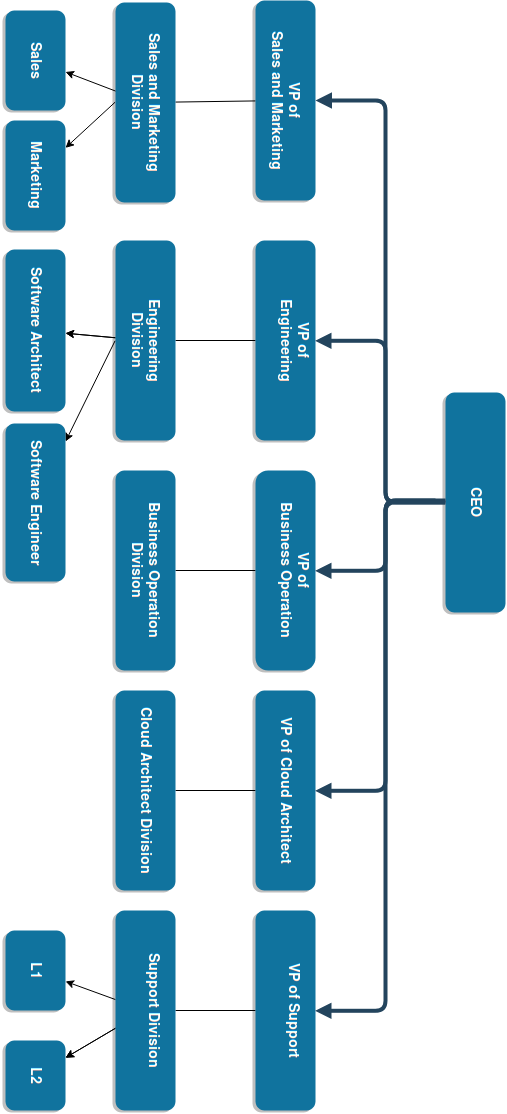
\includegraphics[width=.7\linewidth]{img/struktur-bgn-rotate.png}
  \caption{Struktur Perusahaan Biznet Gio \parencite{biznetgio}}
  \label{fig:struktur-bgn}
\end{figure}


%%% Local Variables:
%%% mode: latex
%%% TeX-master: "pkl"
%%% End:
